% Generated by manuscript/build_manuscript.py.
\section{HoriScope}
\label{sec:method}


Section 3 established two decoder-side requirements for UVHF. Predictions for a shared future target should be invariant to the requested horizon, while the decoder should not impose one latent-state sharing extent on the entire future domain. We address these requirements with \textbf{HoriScope}, an adaptive multi-scope decoder that constructs one future-step-indexed trajectory from multiple sharing granularities. We further develop \textbf{Balanced Scope Co-Adaptation (BSCA)} as the joint optimization strategy for its multi-scope forecast field and allocation process.

\subsection{Architecture overview}


Fig.~\ref{fig:horiscope-method} summarizes the forward computation of HoriScope, which comprises a \textbf{Scope Forecasting Path} and a \textbf{Target-Adaptive Allocation Path}. The decoder consumes a variable-wise History State rather than relying on a particular Encoder. Any Encoder that models temporal patch tokens and returns the required tensor interface can therefore serve as its backbone. This interface covers the patch-based Encoder family commonly used in time-series forecasting \citep{nie2023patchtst,zhang2023crossformer}. Given a History Series $\mathbf X\in\mathbb R^{B\times L\times C}$, Patchify and the Encoder produce $\mathbf R\in\mathbb R^{B\times C\times R}$. The Scope Forecasting Path constructs region-wise predictions under each sharing scope and assembles them into $\mathcal F_\theta(\mathbf X)\in\mathbb R^{B\times C\times T\times S}$. The Target-Adaptive Allocation Path then determines how each future target draws on these sharing granularities.

The Target-Adaptive Allocation Path combines a projected History State with the Future Coordinate $\boldsymbol\phi_\tau$ and produces Scope Probabilities $\boldsymbol\Pi\in\mathbb R^{B\times C\times T\times S}$. Weighted contraction with the scope-indexed forecast field yields one trajectory $\widehat{\mathbf Y}\in\mathbb R^{B\times T\times C}$. For an $H$-step request, HoriScope evaluates the region-target pairs intersecting the first $H$ future steps. Every shared target is generated through the same region-local mapping, irrespective of the requested endpoint. Varying $H$ consequently changes only the output extent, yielding variable-length forecasts that satisfy CHPC by construction.

The Scope-conditioned Forecasts and Scope Probabilities are optimized jointly. BSCA separates two training roles: the Uniform-Prefix Forecasting Loss optimizes varied-horizon prediction, while the Scope-Wise Forecasting Loss and Allocation-Balance Regularizer stabilize multi-scope learning.



\begin{figure*}[t]
\centering
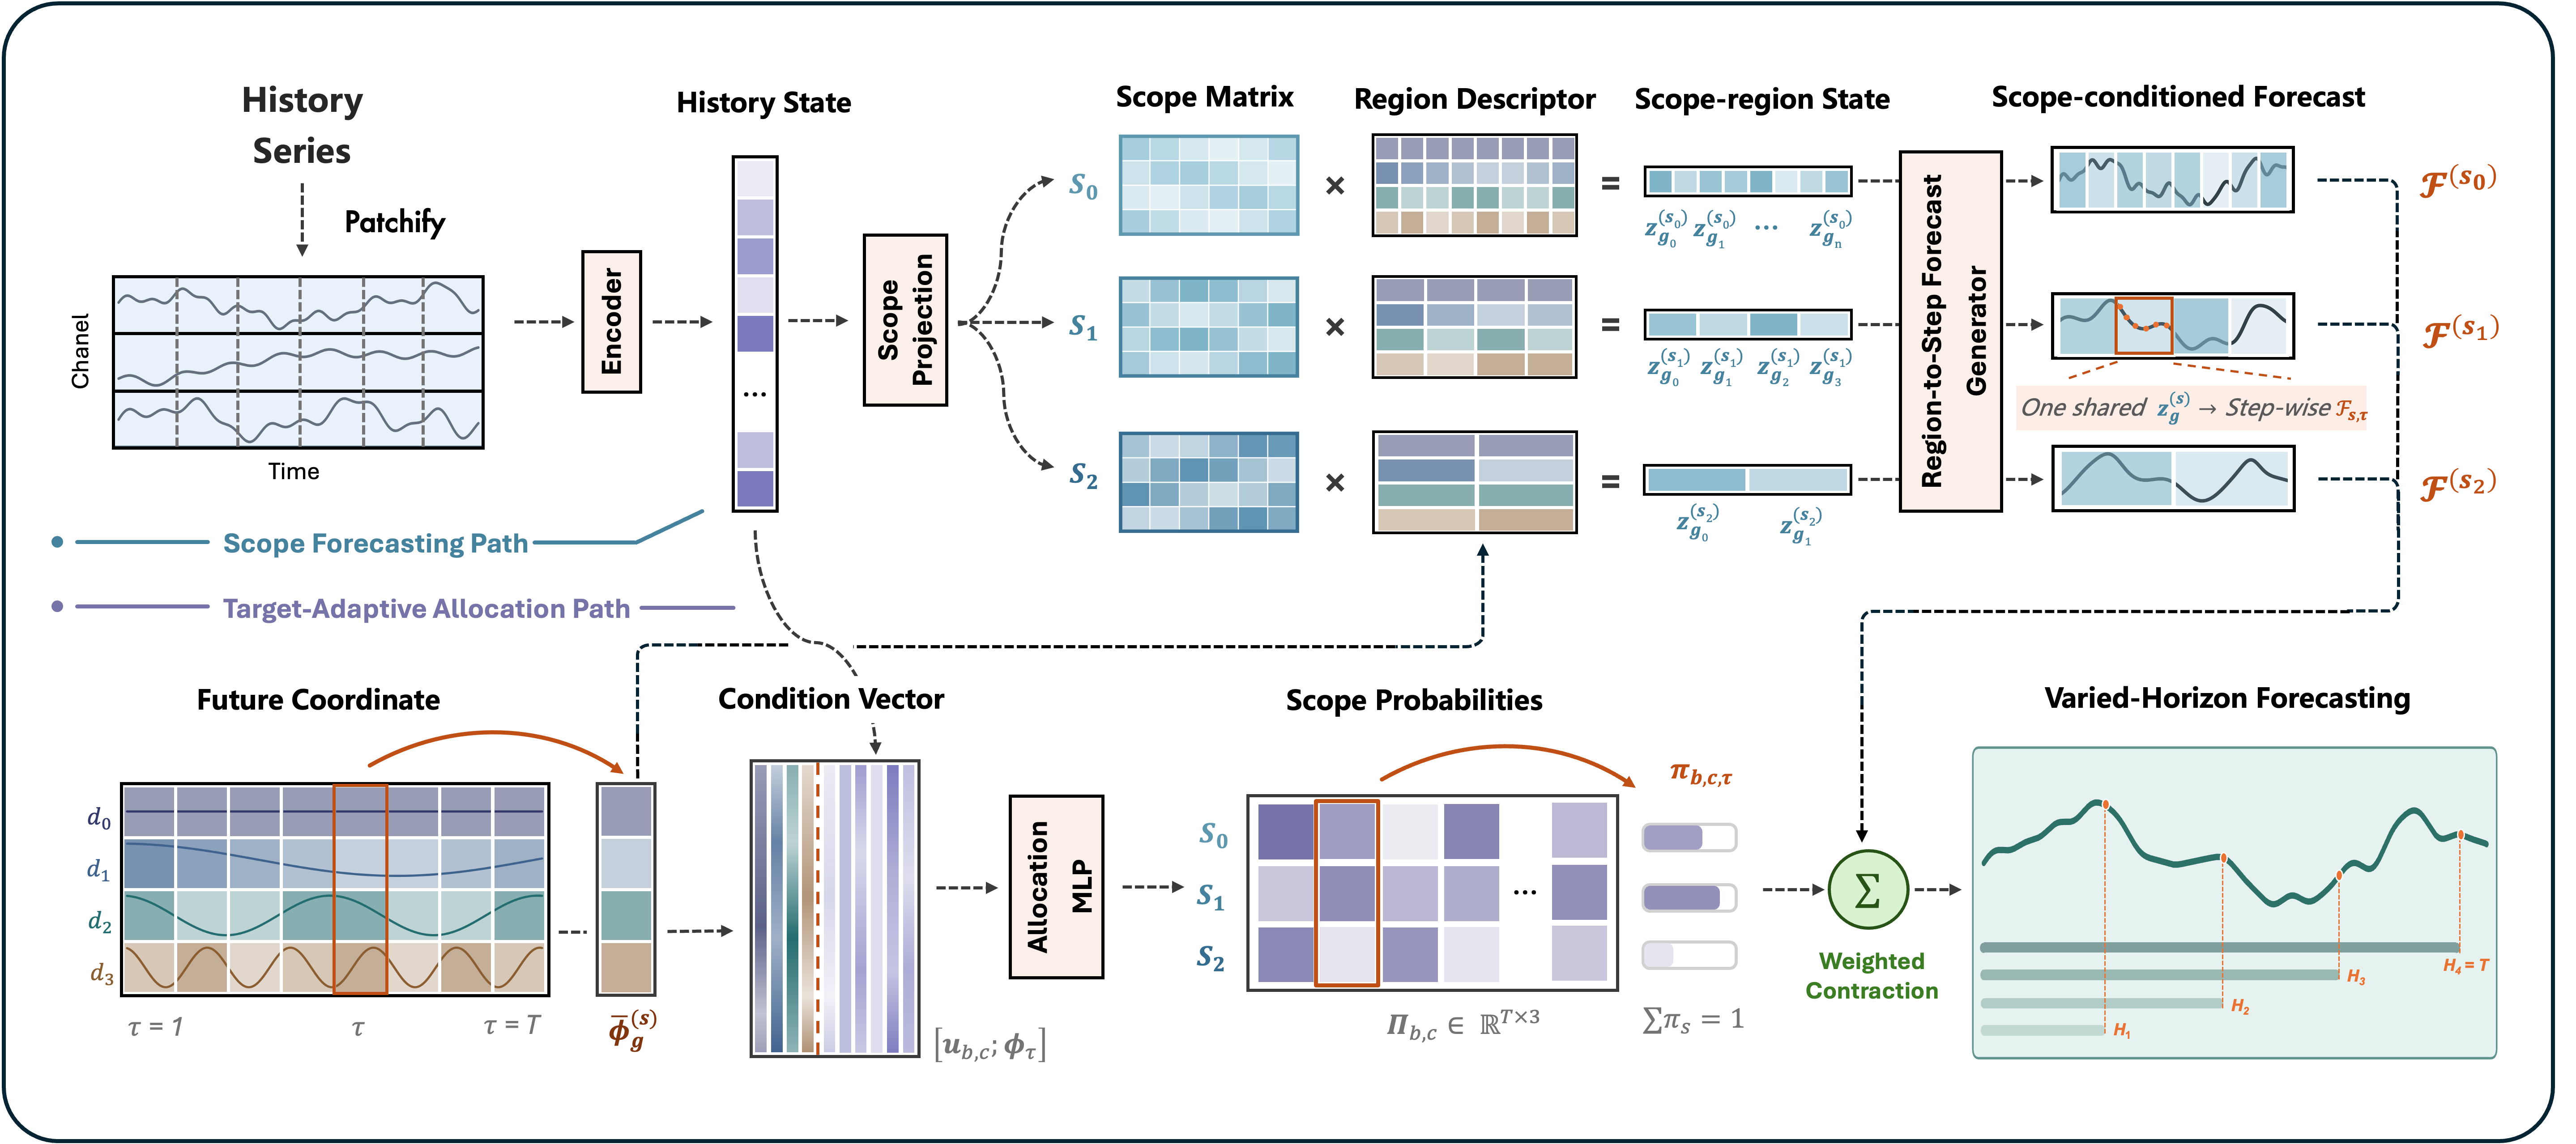
\includegraphics[width=1.00\textwidth]{figures/figure_04_method_overview.png}
\caption{HoriScope for unified varied-horizon forecasting. The Scope Forecasting Path constructs region-wise forecasts under multiple scopes, and the Target-Adaptive Allocation Path combines them into one trajectory whose prefixes serve different horizon requests.}
\label{fig:horiscope-method}
\end{figure*}


\subsection{History state and future coordinate}


HoriScope begins with the History State and Future Coordinate shown on the left of Fig.~\ref{fig:horiscope-method}. The History Series is normalized per variable, divided into $P$ patches by Patchify and processed by the shared Encoder. This produces $\mathbf Z\in\mathbb R^{B\times C\times P\times D_e}$, which is flattened over its patch and embedding dimensions:

\[
\mathbf Z
=
\mathcal E\!\left(\mathcal N(\mathbf X)\right),
\qquad
\mathbf r_{b,c}
=
\operatorname{vec}(\mathbf Z_{b,c})
\in\mathbb R^R,
\qquad
R=PD_e.
\]


Collecting $\mathbf r_{b,c}$ over samples and variables gives the History State $\mathbf R=[\mathbf r_{b,c}]\in\mathbb R^{B\times C\times R}$. The preserved variable axis provides one history representation for each sample-variable pair, which is used by both decoder paths.

The History State summarizes the observed series, but a unified decoder must also identify where each prediction lies in the future domain. Using the requested horizon for this purpose would assign different conditioning contexts to the same target under different requests. HoriScope instead introduces a \textbf{Future Coordinate} for every future step. This fixed coordinate supplies a horizon-independent target identity and a common positional basis for regions at different scopes. It also allows the Target-Adaptive Allocation Path to vary its scope preference across future steps.

Formally, the Future Coordinate is the field $\boldsymbol\Phi=[\boldsymbol\phi_1,\ldots,\boldsymbol\phi_T]^\top\in\mathbb R^{T\times D_q}$. We construct it from low-order discrete cosine functions, which provide smooth coordinate channels at progressively finer temporal frequencies. For $d=0,\ldots,D_q-1$, we first define

\[
\widetilde\phi_{\tau,d}
=
\cos\!\left(
\frac{\pi(\tau-\tfrac12)d}{T}
\right).
\]


The constant coordinate is $\phi_{\tau,0}=1$. Each nonconstant coordinate is centered over the future domain and scaled as

\[
\phi_{\tau,d}
=
\sqrt{2}
\left(
\widetilde\phi_{\tau,d}
-
\frac{1}{T}
\sum_{j=1}^{T}
\widetilde\phi_{j,d}
\right),
\qquad d\geq 1.
\]


The constant channel preserves a global reference, while the centered nonconstant channels distinguish positions across the future domain. The Future Coordinate field serves two roles. Region-wise averaging produces the Region Descriptors used to generate Scope-conditioned Forecasts, whereas the unpooled coordinate $\boldsymbol\phi_\tau$ identifies the individual target in the Condition Vector used for Scope Probabilities.

\subsection{Generation of scope-conditioned forecasts}


The Scope Forecasting Path contains $S$ parallel scope lines, one for each sharing scope in $\mathcal S=\{s_1,\ldots,s_S\}$. Each scope has its own parameterized Scope Projection, which maps the History State into a dedicated Scope Matrix:

\[
\mathbf M_{b,c}^{(s)}
=
\operatorname{reshape}_{D_q\times K}
\left(
\mathbf r_{b,c}\mathbf W^{(s)}
+
\mathbf b^{(s)}
\right)
\in\mathbb R^{D_q\times K}.
\]


The matrix form preserves a Future-Coordinate axis and a latent-mode axis, allowing Region Descriptors to query scope-specific history information at different future locations without assigning a separate prediction head to every region.

For a scope $s$, the future domain is divided into contiguous regions

\[
\mathcal G_g^{(s)}
=
\{(g-1)s+1,\ldots,gs\},
\qquad
g=1,\ldots,T/s.
\]


The Future Coordinate within each region is averaged to form the Region Descriptor, which provides a compact positional summary for region-wise state construction:

\[
\overline{\boldsymbol\phi}_g^{(s)}
=
\frac{1}{s}
\sum_{\tau\in\mathcal G_g^{(s)}}
\boldsymbol\phi_\tau
\in\mathbb R^{D_q}.
\]


The Region Descriptor selects and combines information from this matrix through a coordinate contraction, producing the region-wise Scope-region State

\[
\mathbf z_{b,c,g}^{(s)}
=
\left(\overline{\boldsymbol\phi}_g^{(s)}\right)^\top
\mathbf M_{b,c}^{(s)}
\in\mathbb R^K.
\]


Once the Scope Matrix is available, each Scope-region State depends only on the descriptor of its own region. Regions can therefore be evaluated separately and in parallel, although they draw on the same scope-specific history information. All future steps in $\mathcal G_g^{(s)}$ reuse $\mathbf z_{b,c,g}^{(s)}$. A finer scope constructs more region states and limits reuse to shorter intervals, whereas a broader scope shares each state over a longer interval. Scope therefore defines the cross-step reuse pattern.

The Region-to-Step Forecast Generator converts each shared Scope-region State into step-wise predictions. Let $g_s(\tau)$ denote the region containing step $\tau$. The generator is shared across scopes and regions, and uses step-specific vectors $\mathbf a_\tau,\mathbf n_\tau\in\mathbb R^K$ and bias $\beta_\tau$ to define

\[
\mathcal F_{b,c,\tau,s}
=
\left\langle
\mathbf a_\tau,
\mathbf z_{b,c,g_s(\tau)}^{(s)}
\right\rangle
+
\left\langle
\mathbf n_\tau,
\operatorname{GELU}\!\left(
\mathbf z_{b,c,g_s(\tau)}^{(s)}
\right)
\right\rangle
+
\beta_\tau.
\]


Concatenating the separately generated regions gives the Scope-conditioned Forecast $\mathcal F^{(s)}$ for scope $s$. Collecting these forecasts produces the scope-indexed field $\mathcal F_\theta(\mathbf X)\in\mathbb R^{B\times C\times T\times S}$. Rather than ensembling separately trained models, HoriScope jointly constructs this field through scope-specific projections and a shared Encoder and Region-to-Step Forecast Generator. This design couples forecast generation across scopes while avoiding duplicated Encoder computation and generator parameters.

\subsection{Target-adaptive scope allocation}


Different future targets may require information organized at different sharing granularities. Estimating this preference requires both the dynamics encoded in the observed history and the target position in the future domain. The Target-Adaptive Allocation Path represents these two signals using a compact history summary and the Future Coordinate. It first projects the History State as

\[
\mathbf u_{b,c}
=
\mathbf W_h\mathbf r_{b,c}
+
\mathbf b_h
\in\mathbb R^{D_h}.
\]


The compact summary $\mathbf u_{b,c}$ retains the sample-variable context used for allocation. For future step $\tau$, the Condition Vector concatenates this summary with $\boldsymbol\phi_\tau$. The Allocation MLP maps the resulting vector to scope logits

\[
\boldsymbol\ell_{b,c,\tau}
=
\mathbf W_o
\operatorname{GELU}\!\left(
\mathbf W_p
[\mathbf u_{b,c};\boldsymbol\phi_\tau]
+
\mathbf b_p
\right)
+
\mathbf b_o
\in\mathbb R^S,
\]


\[
\pi_{b,c,\tau,s}
=
\frac{
\exp(\ell_{b,c,\tau,s})
}{
\sum_{s'=1}^{S}
\exp(\ell_{b,c,\tau,s'})
}.
\]


Softmax converts these logits into the Scope Probability $\pi_{b,c,\tau,s}$ assigned to scope $s$. Collecting all probabilities gives $\boldsymbol\Pi\in\mathbb R^{B\times C\times T\times S}$, with $\sum_{s=1}^{S}\pi_{b,c,\tau,s}=1$. Each probability vector parameterizes how strongly a future target draws on information organized at different sharing granularities. The final normalized prediction reads from the unified scope-indexed forecast field through weighted contraction:

\[
\widehat y_{b,\tau,c}
=
\sum_{s=1}^{S}
\pi_{b,c,\tau,s}
\mathcal F_{b,c,\tau,s}.
\]


This contraction is not an average over separately trained model outputs. The Scope Forecasting Path and Target-Adaptive Allocation Path are jointly learned within one decoder, allowing each target to receive a history-conditioned mixture of sharing granularities.

For an $H$-step request, HoriScope needs only the Scope-region States whose regions intersect $1{:}H$ and the allocation entries for $\tau\leq H$. The resulting normalized prefix is transformed back to the original data scale and returned as

\[
\widehat{\mathbf Y}_b^{(H)}
=
\left[
\widehat y_{b,\tau,c}
\right]_{\tau=1,\ldots,H;\ c=1,\ldots,C}.
\]


Changing $H$ restricts the active region and target computations but does not alter any prediction shared with a longer request. Every request is therefore a nested view of the same trajectory. The learned probabilities represent target-adaptive information allocation rather than an oracle scope selector. Later ablations and internal-behavior analyses evaluate whether this allocation yields useful scope differentiation.

\subsection{Balanced Scope Co-Adaptation}


Training HoriScope introduces two coupled requirements. The fused trajectory requires uniform supervision across supported prefix lengths, while all scope lines must develop reliable forecasts as allocation is learned. BSCA therefore combines the \textbf{Uniform-Prefix Forecasting Loss} for varied-horizon prediction with two terms that stabilize multi-scope learning: the \textbf{Scope-Wise Forecasting Loss} and \textbf{Allocation-Balance Regularizer}.

Varied-horizon training should optimize every supported prediction length without privileging one endpoint. We therefore average raw-scale MAE equally over all prefixes $h=1,\ldots,T$ to define the Uniform-Prefix Forecasting Loss. Before loss evaluation, inverse normalization maps the fused and Scope-conditioned Forecasts to the original data scale. Let $y_{b,\tau,c}$ denote the corresponding raw-scale target. The fused objective is

\[
\mathcal L_{\mathrm{prefix}}
=
\frac{1}{T}
\sum_{h=1}^{T}
\frac{1}{BCh}
\sum_{b=1}^{B}
\sum_{c=1}^{C}
\sum_{\tau=1}^{h}
\left|
\widehat y_{b,\tau,c}-y_{b,\tau,c}
\right|.
\]


Exchanging the prefix and future-step summations gives an equivalent dense-prefix measure

\[
\omega_\tau
=
\frac{1}{T}
\sum_{h=\tau}^{T}
\frac{1}{h},
\qquad
\sum_{\tau=1}^{T}\omega_\tau=1.
\]


Under this measure, every prefix endpoint contributes equally, while a future step is weighted by the number of prefixes containing it. The same loss can therefore be written as

\[
\mathcal L_{\mathrm{prefix}}
=
\frac{1}{BC}
\sum_{b=1}^{B}
\sum_{c=1}^{C}
\sum_{\tau=1}^{T}
\omega_\tau
\left|
\widehat y_{b,\tau,c}-y_{b,\tau,c}
\right|.
\]


The Uniform-Prefix Forecasting Loss establishes the varied-horizon objective, but it does not resolve the joint optimization of multiple scope lines. Weighted contraction makes the fused-loss gradient received by each scope depend on its current Scope Probability. For a fixed target, this relation gives

\[
\frac{
\partial\mathcal L_{\mathrm{prefix}}
}{
\partial\mathcal F_{b,c,\tau,s}
}
=
\pi_{b,c,\tau,s}
\frac{
\partial\mathcal L_{\mathrm{prefix}}
}{
\partial\widehat y_{b,\tau,c}
}.
\]


Consequently, early probability concentration can suppress learning in low-probability scope lines before their forecasts mature. The allocator then compares unevenly developed predictions, which can reinforce its initial preference. We first address this imbalance with the Scope-Wise Forecasting Loss, which applies the same prefix measure directly to every Scope-conditioned Forecast:

\[
\mathcal L_{\mathrm{scope}}
=
\frac{1}{BCS}
\sum_{b=1}^{B}
\sum_{c=1}^{C}
\sum_{s=1}^{S}
\sum_{\tau=1}^{T}
\omega_\tau
\left|
\mathcal F_{b,c,\tau,s}-y_{b,\tau,c}
\right|.
\]


This term gives every scope a direct prediction gradient independent of its current Scope Probability. Direct supervision alone, however, does not regulate how the fused predictor distributes probability-mediated gradients. We therefore introduce the Allocation-Balance Regularizer using the uniform reference $q_s=1/S$:

\[
\mathcal L_{\mathrm{balance}}
=
\frac{1}{BC}
\sum_{b=1}^{B}
\sum_{c=1}^{C}
\sum_{\tau=1}^{T}
\omega_\tau
\frac{
D_{\mathrm{KL}}\!\left(
\mathbf q\,\Vert\,\boldsymbol\pi_{b,c,\tau}
\right)
}{
\log S
}.
\]


The complete objective is

\[
\mathcal L_{\mathrm{BSCA}}
=
\mathcal L_{\mathrm{prefix}}
+
\lambda_{\mathrm{scope}}
\mathcal L_{\mathrm{scope}}
+
\lambda_{\mathrm{balance}}(u)
\mathcal L_{\mathrm{balance}},
\]


where $u\in[0,1]$ is optimizer progress. In the frozen configuration, $\lambda_{\mathrm{scope}}=1$ and

\[
\lambda_{\mathrm{balance}}(u)
=
0.1
\min\!\left(
\frac{u}{0.25},1
\right).
\]


The regularizer penalizes strongly non-uniform Scope Probabilities, discouraging a small subset of scopes from dominating early optimization. Its ramp introduces this pressure gradually as the forecasting paths develop. This pressure promotes broader allocation and a more even distribution of probability-mediated gradients across scope lines. Together with direct scope supervision, it supports more balanced multi-scope optimization.
